%%%%%%%%%%%%%%%%%%%%%%%%%%%%%%%%%%%%%%%%%%%%%%%%%%%%%%%%%%%%%%%%%%%%%%%%%%%%%%%
% Seismica submission manuscript -- shortened main paper, version 39
% Supporting detail and diagnostic figures are in supplement39.tex.
%%%%%%%%%%%%%%%%%%%%%%%%%%%%%%%%%%%%%%%%%%%%%%%%%%%%%%%%%%%%%%%%%%%%%%%%%%%%%%%

\documentclass[]{seismica}
\usepackage{tabularx}
\usepackage{placeins}

% Compile from the repository latex/ directory.
\graphicspath{
  {../data/outputs/170_generate_publication_figures/}
  {../data/outputs/165_generate_video_waveform_figure/}
  {../data/outputs/145_analyze_regional_detectability/}
  {../data/outputs/140_search_for_direct_seismic_waves/}
  {../data/outputs/130_analyze_seismic_polarization/}
  {../data/outputs/120_estimate_acoustic_energetics/}
  {../data/outputs/110_measure_named_events/}
  {../data/outputs/100_measure_event_amplitudes_and_acoustic_seismic_coupling/figures/}
  {../data/outputs/100_measure_event_amplitudes_and_acoustic_seismic_coupling/}
  {../data/outputs/090_analyze_finite_distance_propagation/}
  {../data/outputs/080_analyze_planar_array_propagation/}
  {../data/outputs/040_validate_event_catalogue_with_array_processing/figures/}
  {figures/}
}

% These boxes keep the manuscript compilable while the two remaining main
% figures are regenerated. They should not appear in a submitted PDF.
\newcommand{\pendingfigure}[1]{%
  \fbox{\parbox[c][55mm][c]{0.92\textwidth}{\centering\textbf{Pending figure}\par#1}}}

\title{Close-Range Seismo-Acoustic Observations of the 2016 Falcon 9 AMOS-6 Failure at Cape Canaveral}
\shorttitle{Close-range observations of the 2016 Falcon 9 explosion}

% Confirm department-level present affiliations for Farrell and Mehta before
% submission.
\author[1]{Glenn Thompson\thanks{Corresponding author: \texttt{thompsong@usf.edu}; ORCID: 0000-0002-9173-0097}}
\author[2,3]{Robert G. Brown}
\author[1,4]{Alexandra Farrell}
\author[2,3]{John Kiriazes}
\author[1]{Stephen R. McNutt}
\author[1,5]{Christopher Mehta}
\affil[1]{School of Geosciences, University of South Florida, Tampa, Florida, USA}
\affil[2]{NASA Kennedy Space Center, Florida, USA}
\affil[3]{Present address: Florida Space Institute, University of Central Florida, Orlando, Florida, USA}
\affil[4]{Present address: University of Alaska Fairbanks, Fairbanks, Alaska, USA}
\affil[5]{Present address: Howard University, Washington, DC, USA}

\credit{Conceptualization}{Glenn Thompson}
\credit{Methodology}{Glenn Thompson}
\credit{Software}{Glenn Thompson}
\credit{Validation}{Glenn Thompson}
\credit{Formal Analysis}{Glenn Thompson}
\credit{Investigation}{Glenn Thompson, Robert G. Brown, Alexandra Farrell,
John Kiriazes, Stephen R. McNutt, Christopher Mehta}
\credit{Resources}{Robert G. Brown, John Kiriazes}
\credit{Data Curation}{Glenn Thompson}
\credit{Visualization}{Glenn Thompson}
\credit{Project Administration}{Glenn Thompson, Robert G. Brown}
\credit{Writing - Original draft}{Glenn Thompson}
\credit{Writing - Review \& Editing}{Glenn Thompson, Robert G. Brown,
John Kiriazes, Stephen R. McNutt}

\begin{document}

\makeseistitle{
  \begin{summary}{Abstract}
  On 1 September 2016, a Falcon~9 and its AMOS-6 payload were destroyed
  during propellant loading before a planned static-fire test at Space Launch
  Complex~40, Cape Canaveral. A broadband seismometer and three-element
  infrasound array 1.4~km away recorded the complete sequence. We reconstructed
  its chronology, screened a continuous 48-h record for conspicuous
  multichannel impulsive precursors, and measured source direction,
  propagation, pressure, ground motion, and acoustic--seismic coupling. The
  catalogue contains 153 accepted pressure transients in four phases over
  26~min. No precursor signal was found in the seismo-acoustic data before
  the initial upper-stage explosion. The principal explosion followed the initial
  upper-stage event by about 3.6~s and produced median positive and
  peak-to-peak pressures of about 1.4 and 1.6~kPa, respectively. Its positive-peak sound
  pressure level was about 157~dB relative to the standard 20-$\mu$Pa
  reference pressure, and its median hemispherical radiated acoustic-energy
  estimate was $2.2\times10^9$~J. High-quality array solutions pointed toward
  the launch complex and gave an apparent velocity of about
  352~m~s$^{-1}$, consistent with meteorological predictions. Pressure and
  three-component peak ground velocity were nearly proportional across 46
  well-measured events.
  \end{summary}
  %
  \begin{summary}{Non-technical summary}
  A seismic and low-frequency sound station approximately 1.4~km from the
  launch pad recorded the 2016 Falcon~9 accident at Cape Canaveral. The
  recordings independently show when energetic activity began, how the
  sequence developed, how large its strongest signals were, and whether the
  pressure waves were consistent with propagation from the launch complex. A
  gap-free 48-h record, spanning 37~h before and 11~h after the first signal,
  was examined on all six channels, with no precursor signal identified before
  the initial upper-stage explosion.
  The accident was not a single explosion: 153 accepted multichannel pressure
  transients occurred in four phases over approximately 26~min, although some
  closely spaced entries are different peaks within the same physical event
  complex. The strongest explosion followed the first upper-stage signal by
  about 3.6~s. Independent measurements of arrival direction and speed agree with
  propagation from the launch pad under the observed weather conditions. The
  study shows that a small continuously recording geophysical array can
  provide an empirically calibrated, independently timed forensic record when access to a
  launch site is restricted and engineering telemetry is unavailable.
  \end{summary}
}

\section{Introduction}
\label{sec:introduction}

Rocket launches generate strong atmospheric and ground-motion signals, but
catastrophic launch failures are rarely recorded at close range by calibrated
seismic and infrasound instruments. Most seismo-acoustic studies of major
technological explosions have instead used regional observations, for which
atmospheric ducting and attenuation strongly influence arrival times and
amplitudes \citep{ottemoller_2008,green_2008,ceranna_2009,smink_2019,
pilger_beirut_2021,kim_pasyanos_2022}. Rocket-focused studies demonstrate
complementary capabilities: routine launches are detectable infrasonically at
large distances \citep{pilger_rocket_2021}, dense seismic deployments can
resolve launch-generated body and surface waves
\citep{schuster_rocketquake_2025}, and regional infrasound can locate and
estimate the effective yield of a large static-fire explosion
\citep{silber_scamfer_newglenn_2026}.

On 1 September 2016, a Falcon~9 was destroyed during propellant loading in the
countdown for a planned static-fire test at Space Launch Complex~40 (SLC-40),
Cape Canaveral Air Force Station (now Cape Canaveral Space Force Station),
Florida. The AMOS-6 payload was lost and the launch complex was extensively
damaged. The only publicly available original recording is the 5-min-40-s raw
USLaunchReport video and camera audio \citep{uslaunchreport_amos6_video_2016};
an edited analysis by \citet{manley_spacex_explosion_2016} was used only for
context.

The University of South Florida (USF) BCHH station, approximately 1.4~km from
SLC-40 on adjacent Kennedy Space Center property, fortuitously recorded the
complete sequence. The initial forensic analysis was documented in an
unpublished USF technical report prepared for SpaceX in November~2016
\citep{thompson_mcnutt_fireball_2016} and subsequently presented publicly at
the 2017 AGU Fall Meeting \citep{thompson_agu_falcon9_2017}, before the
present reanalysis. The geophysical chronology was developed independently of
the later engineering root-cause determination.

The central advantage of this dataset is the combination of continuous
recording, physical calibration, array geometry, and proximity. It permits
subsecond timing and local pressure--ground comparisons that are usually
unavailable at regional distances, while public imagery provides an
independently inspectable record of selected physical stages. It also exposes
important limitations: one compact array can constrain direction and apparent
speed but not source range, and it cannot assign every later transient to a
specific vehicle or pad component.

Here we use the BCHH observations to test for a detectable energetic
precursor, reconstruct the accident chronology, measure the strongest events,
evaluate source direction and acoustic propagation, and characterize local
pressure--ground coupling. A separate regional search tests whether the
principal explosion can be associated with publicly archived records at much
greater distances. The broader objective is to establish which forensic
inferences a modest open geophysical deployment can support independently and
which still require engineering telemetry, denser spatial sampling, or
detailed atmospheric modelling at this unusual observational scale. We use
\emph{close range}, rather than the strict
acoustic term \emph{near field}: a 1.4-km wavelength at 350~m~s$^{-1}$
corresponds to approximately 0.25~Hz, below the principal analysis band.
Supporting methods, diagnostics, and sensitivity results are provided in the
Supplementary Material.

\section{Data and instrumentation}
\label{sec:data}

\subsection{BCHH array and geometry}

BCHH comprised a three-component Nanometrics Trillium Compact Posthole
seismometer near the centre of a three-element infraBSU pressure array with an
aperture of approximately 30~m (Figure~\ref{fig:site_array}). All six channels
were recorded continuously at 250~Hz by a GPS-synchronized Nanometrics
Centaur. The seismometer was buried approximately 0.5~m; the pressure sensors
were mounted 20--30~cm above ground.

On 6 October 2016, as Hurricane Matthew approached KSC, co-author Robert G.
Brown removed the three pressure sensors, electronics enclosures, and solar
panels; the buried seismometer remained in place. Because the pressure sensors
had not been formally surveyed before their precautionary removal, their
geometry was subsequently reconstructed from the surveyed cable-end locations.
Relative position errors of approximately 1--2~m are therefore plausible.
Source distances ranged from 1408.3 to 1440.0~m
(Supplementary Table~S1). DD2 was used as the reference
pressure channel.

\begin{figure*}[!tbp]
  \centering
  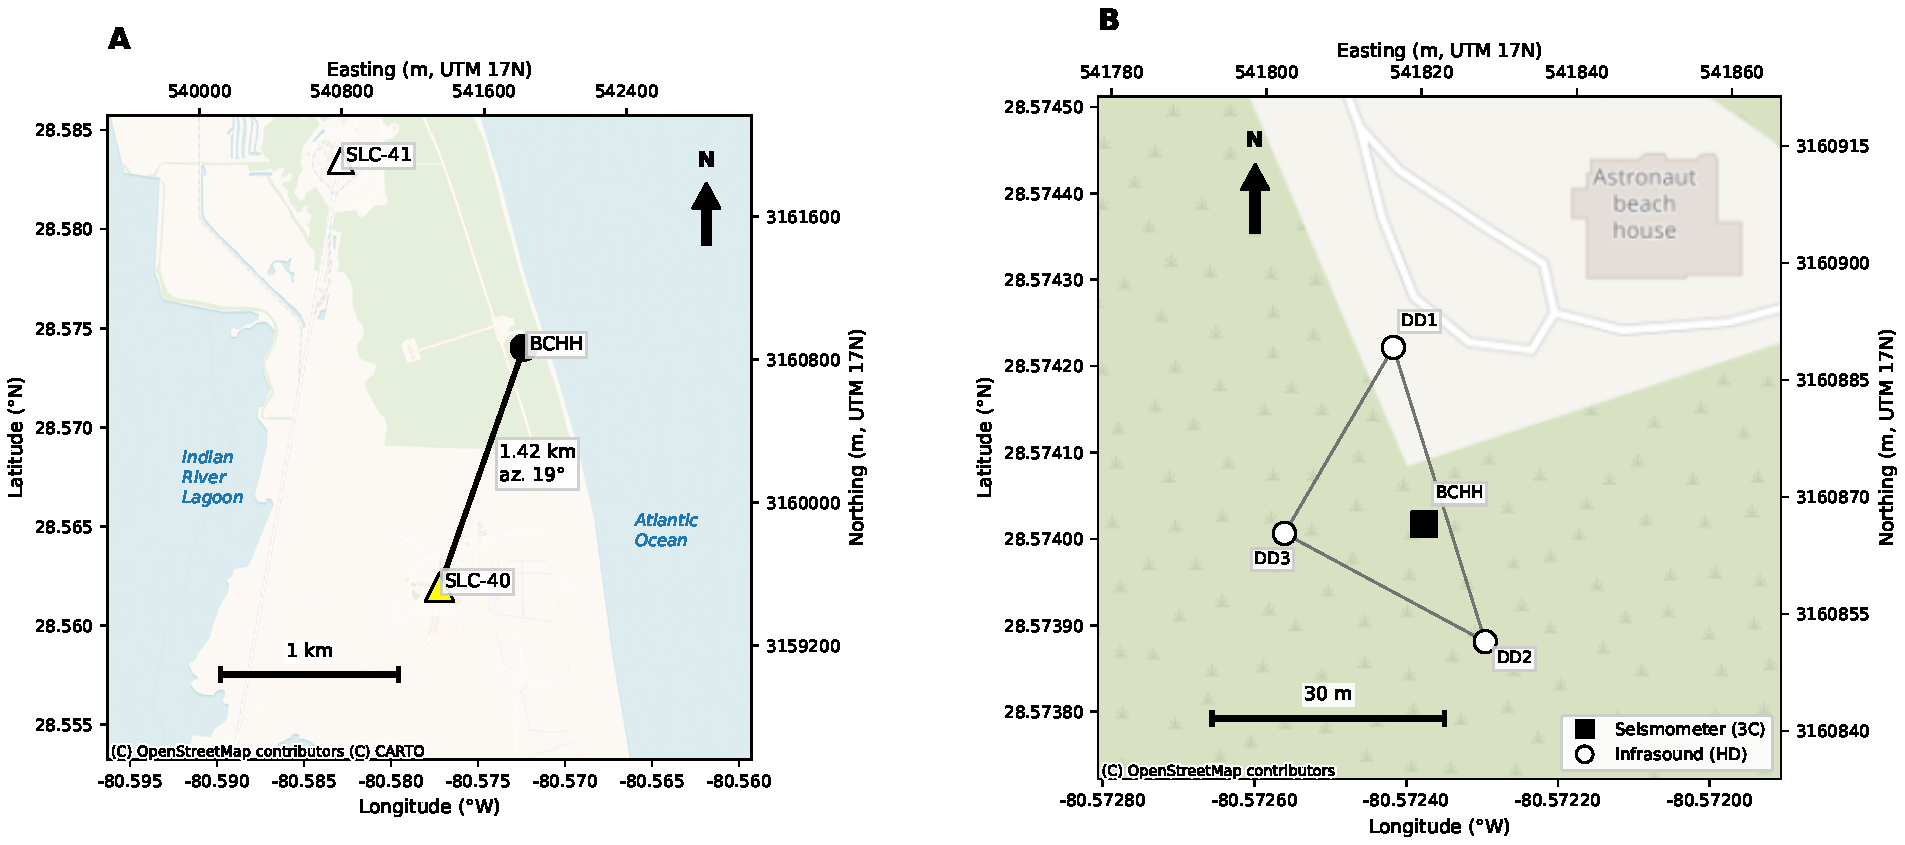
\includegraphics[width=0.96\textwidth]{fig01_slc40_bchh_location.pdf}
  \caption{Location and geometry of the BCHH seismo-acoustic array.
  (a) SLC-40 and BCHH in the southern Kennedy Space Center--Cape Canaveral
  launch area. (b) Three-component seismometer and three-element infrasound
  array. Pressure-sensor positions were reconstructed from surveyed cable ends,
  giving metre-scale relative-position uncertainty.}
  \label{fig:site_array}
\end{figure*}
\FloatBarrier

\subsection{Calibration, weather, video, and regional data}

The seismic response was removed using the manufacturer calibration for the
Trillium Compact Posthole--Centaur chain. Field checks during the 2015
Sakurajima campaign identified sensitivities differing from the common
nominal conversion subsequently used in the published analysis
\citep{smith_sakurajima_2020}; these observations motivated the KSC calibration
experiments. The inventory included several All Sensors pressure-transducer
ranges with different nominal sensitivities. The November~2016 forensic
report documents BCHH lift-test factors of 0.1234, 1.45, and
0.100~Pa~count$^{-1}$ for DD1--DD3, equivalent to 8.10, 0.690, and
10.0~counts~Pa$^{-1}$, respectively \citep{thompson_mcnutt_fireball_2016}.
These empirical factors are retained here (Supplementary Table~S1).
DD1 and DD3 are consistent with 1-inch H$_2$O heads, but channel-to-head
assignments and the cause of DD2's lower sensitivity remain unresolved.
The available evidence does not establish incorrect calibration when supplied.
Supplementary Section~S1 describes the historical tests and their limitations.
The provisional $\pm20\%$ pressure uncertainty reflects empirical test
variability rather than a laboratory-traceable absolute uncertainty. Manual
arrival uncertainty was approximately 0.01~s for the clearest impulses and
greater for weak, emergent, or overlapping signals.

The USLaunchReport footage provided the public visual and camera-audio record.
Four proprietary videos obtained from SpaceX assisted and confirmed visual
interpretation but contained no usable audio and supplied no quantitative
result reported here. Data were sought from an infrasound array at CCAFS
operated by the Air Force Technical Applications Center (AFTAC)
but were ultimately reported to have been lost. Regional pressure records to 1800~km
and vertical seismic records to 600~km were obtained through EarthScope FDSN
services; IU.DWPF, 97.7~km from SLC-40, was the nearest permanent station
examined \citep{asl_gsn_iu_1988}.

Kennedy Space Center weather-tower observations supplied temperature,
relative humidity, and wind profiles at seven 5-min epochs from 13:05 to
13:35~UTC. Across the available observations, mean temperature was
26.4$\pm0.3\,^{\circ}$C and mean relative humidity was
83.9$\pm3.7\%$. The overall vector-mean wind was 5.4~m~s$^{-1}$ from
144$^\circ$, varying little among the seven epochs (5.3--5.5~m~s$^{-1}$,
142--149$^\circ$).
Atmospheric profiles and temporal variability are shown in Supplementary
Figures~S1 and~S2.

\FloatBarrier

\section{Methods}
\label{sec:methods}

The analysis was implemented in Python as a reproducible sequence of Jupyter
notebooks \citep{kluyver2016jupyter}. Shared configuration and intermediate
products supplied common geometry, event times, propagation corrections, and
analysis parameters. Additional implementation and sensitivity details are in
Supplementary Sections~S1--S7.

\subsection{Waveform preparation and meteorological reduction}

Response removal used a 0.02, 0.05, 80, and 100~Hz four-corner prefilter and a
60-dB water level. A centred 1.0-s moving median was then removed independently
from each pressure channel to suppress slow baseline variation without an
additional physical-amplitude high-pass filter. Seismic traces remained in
ground velocity and pressure traces in Pa.

Using the mean temperature and humidity described in Section~2.2, the
still-air sound speed was 348.3~m~s$^{-1}$. Wind vectors were projected onto
the SLC-40--BCHH propagation direction. The available lower-atmosphere profile,
summarized over the nominal 0--65-m source-height interval, gave a vector-mean
wind of 4.6~m~s$^{-1}$ from 145$^\circ$ and a path-parallel tailwind component
of 2.6~m~s$^{-1}$. Because the lowest valid wind observations were near 40~m,
this lower-path estimate does not directly sample the entire surface layer.
Effective acoustic speed was calculated as
\begin{equation}
 c_{\mathrm{eff}}=c_0+\mathbf{u}\boldsymbol{\cdot}\hat{\mathbf{r}}.
 \label{eq:effective_speed}
\end{equation}
The calculated effective acoustic speed was 351.0~m~s$^{-1}$, which was used
for source-to-BCHH travel-time reduction.
Three time coordinates were kept distinct: observed
receiver UTC, DD2-referenced reduced arrival time, and source time. For sensor
$i$,
\begin{equation}
 t_{i,\mathrm{red}}=t_i-\frac{r_i-r_{\mathrm{DD2}}}{c_{\mathrm{eff}}}.
 \label{eq:reduced_time}
\end{equation}
Thus, catalogue times used for event association represent arrivals reduced
to DD2. Source times were calculated separately by subtracting the complete
source-to-DD2 acoustic travel time.

\subsection{Catalogue construction and quality control}

A gap-free 48-h interval extending from 37~h before to 11~h after the first
upper-stage signal was manually scanned by the lead author (GT) using
Antelope's \texttt{dbpick} program (version~5.6) \citep{brtt_antelope}. All three pressure and all three seismic
channels were viewed together. GT marked conspicuous impulsive signals readily
visible across the compact array; isolated local disturbances, including
possible vehicle passages, occurred elsewhere but were not treated as
accident-related events.

For association, each pressure pick was first reduced to the DD2 reference by
subtracting the predicted differential travel time from SLC-40 to that sensor
using the 351~m~s$^{-1}$ effective acoustic speed. Picks were then grouped when
at least two pressure channels agreed within 0.04~s, the smallest coincidence
window on a stable association-count plateau. A short MATLAB/GISMO workflow
implemented this grouping \citep{thompson_gismo_2017}; because the candidate
impulses had already been isolated manually, the procedure formalized
cross-channel association rather than recovering marginal signals. Candidate
waveforms were subsequently reviewed for signal-to-noise ratio (SNR),
correlation, and a coherent counterpart on the remaining channel. The
catalogue records accepted multichannel pressure transients, not independently
verified physical explosions.

Catalogue membership was separated from waveform quality. DD1 was
sporadically noisier and, overall, correlated less consistently with the other
two pressure channels; DD2 and DD3 therefore provided the most stable
waveform-quality pair. The usable-waveform subset required robust peak
SNR $\geq3$ and DD2--DD3 correlation $\geq0.5$; the core subset required
SNR $\geq5$ and correlation $\geq0.7$. Time-domain propagation quality was classified independently of
these waveform criteria. The high-quality planar class required maximum
coherence $\geq0.90$, back-azimuth standard deviation
$\leq0.5^\circ$, and apparent-speed standard deviation
$\leq3.0$~m~s$^{-1}$ across nine perturbations of the event scoring window.
Intermediate solutions used corresponding thresholds of 0.75,
1.0$^\circ$, and 8.0~m~s$^{-1}$.

Independent frequency-domain Bartlett beamforming was performed with LANL
InfraPy version~0.4.1.0 \citep{webster_infrapy_2025}, using all three pressure
channels. The primary validation used 0.5-s windows centred on the catalogue
times and a 2--20-Hz band. If $C$ is multichannel coherence for $N=3$
sensors, the Bartlett detection statistic was
\begin{equation}
 F=\frac{(N-1)C}{1-C}.
\end{equation}
This monotonic transformation of coherence is used here as a measure of how
strongly a window supports a coherent plane wave across the array: larger
$F$ means greater intersensor coherence, not greater pressure, energy, or
yield. An empirical detection threshold was defined as the 99.5th percentile
of 153 pre-event background windows, corresponding to $F=3.02$. Event-centred
$F$ values therefore provide an independent array-coherence check on catalogue
entries, while a separate scan of 17,839 overlapping windows, positioned
without reference to catalogue times, tested catalogue recovery and searched
for additional coherent activity.

\subsection{Propagation, amplitude, and coupling analyses}

A time-domain planar-wave grid search estimated back azimuth and apparent
velocity by maximizing multichannel waveform agreement. All catalogue entries
were processed, while physical interpretation emphasized quality-controlled
solutions. A fixed-source circular-wavefront calculation tested sensitivity to
the 1.4-km source range; because the three-element array provides only two
independent relative delays, it was not expected to resolve both source range
and propagation speed.

For each event, peak-to-peak pressure was measured from the differentially
aligned channels and three-component vector peak ground velocity (PGV) was
measured over a pressure-defined seismic window. A log--log model
\begin{equation}
 \log_{10}p_{\mathrm{p2p}}=a+b\log_{10}(\mathrm{PGV})
 \label{eq:power_law}
\end{equation}
was fitted to catalogue entries satisfying separate pressure-SNR, seismic-SNR,
and window-capture criteria; uncertainty was estimated by catalogue-entry
bootstrap. Because closely spaced entries can belong to one physical event
complex, this interval does not account for within-complex dependence.

Frequency-dependent coupling was described by the H1 pressure-to-vertical-velocity estimator
\begin{equation}
 H_1(f)=\frac{S_{pv}(f)}{S_{pp}(f)},
 \label{eq:h1_transfer}
\end{equation}
with magnitude-squared coherence and permutation-derived empirical null
thresholds. Continuous estimates used the opening activity interval
(Phase~I, 13:07:11.91--13:08:21.91~UTC; see Section~\ref{sec:temporal_evolution}).
Event and continuous estimates overlap in time and were treated as
complementary rather than independent.

For the four video-interpreted opening signals later listed in
Table~\ref{tab:principal_events}---the upper-stage event, principal explosion,
candidate payload impact, and payload-associated explosion---acoustic exposure
was integrated over manually reviewed windows. Assuming hemispherical
radiation without atmospheric attenuation,
\begin{equation}
 E_{2\pi}=\frac{2\pi r^2}{\rho c}\int p^2(t)\,dt.
 \label{eq:acoustic_energy}
\end{equation}
Acoustic TNT equivalence is $E_{2\pi}/(4.184\times10^6~\mathrm{J\,kg^{-1}})$,
an energy-unit conversion rather than a blast-yield estimate. Converting
radiated acoustic energy to total explosive yield additionally requires the
acoustic efficiency---the fraction of the source energy radiated into the
atmosphere as sound---which depends on source physics, confinement, and
frequency content and is not constrained by this single close-range station.
Empirical regional period--yield relations used in other explosion studies
avoid specifying that efficiency explicitly because they are calibrated
against explosions of known yield, but no confirmed regional Falcon~9 branch
with a stable dominant period was available here. Overlapping catalogue
windows were not summed as independent events. Efficiency-dependent
total-energy scenarios are therefore confined to the Supplementary Material.

\subsection{Video alignment and regional screening}

The USLaunchReport recording lacks absolute UTC timing. Its first visible upper-stage
flash was mapped to the independently reduced BCHH chronology. Camera audio
was advanced by its 12.16-s path travel time, calculated from a 4.255-km range
and a camera-path effective speed of 349.8~m~s$^{-1}$. BCHH traces were reduced
using sensor-specific distances and 351~m~s$^{-1}$. Video supplied physical
labels for selected stages but was not used to construct the general catalogue.

Regional screening used broad physically plausible acoustic-celerity and
seismic-velocity windows. Candidate windows had to exceed matched pre- and
post-event controls and were then reviewed manually. Association required a
physically consistent multi-station branch; missing data or response failures
were not counted as non-detections.

\section{Results}
\label{sec:results}

\subsection{Atmosphere, catalogue, and temporal evolution}
\label{sec:temporal_evolution}

The meteorological reduction gave an effective acoustic speed of
351.0~m~s$^{-1}$, corresponding to a travel time of approximately 4.05~s over
the 1419.9-m source-to-seismometer distance, about 0.03~s shorter than the
still-air estimate.

The final catalogue contains 153 accepted multichannel pressure transients:
48 in Phase~I, 4 in Phase~II, 96 in Phase~III, and 5 in Phase~IV
(Figure~\ref{fig:overview}). The phases are descriptive intervals enclosing
visually separated activity clusters: Phase~I, 13:07:11.91--13:08:21.91;
Phase~II, 13:14:05--13:15:55; Phase~III, 13:19:02--13:25:00; and Phase~IV,
13:29:39--13:34:54~UTC. They are not inferred source regimes. Of the 153
entries, 138 met usable-waveform and 107 met core
criteria. The independently defined planar classes contained 51 high-quality,
45 intermediate, and 57 weak or broad solutions. Median robust peak SNR was
7.86, median DD2--DD3 correlation 0.876, and median corrected span among
associated picks 4.87~ms. These nested counts serve different analytical
purposes and should not be interpreted as counts of independent explosions.

No precursor signal was identified in the seismo-acoustic data during the
37~h before the initial upper-stage explosion. The visual screen was sensitive
to signals comparable to the accepted array-wide events
under the observed background; it cannot exclude weak, spatially local,
non-impulsive, internal, or otherwise poorly coupled processes. No additional
explosion-related impulse was found in the remainder of the 48-h review window,
which extends approximately 10.5~h beyond Phase~IV. A prolonged signal lasting
approximately 3.2~min followed Phase~I; it is visible on DD2 pressure as well
as the seismic channels, and its source is not uniquely resolved.

\begin{figure*}[!tbp]
  \centering
  \includegraphics[width=0.98\textwidth]{fig03_bchh_30min_overview_zp_true.pdf}
  \caption{Thirty-minute six-channel helicorder-style BCHH overview. The upper
  traces are pressure and the lower traces are three-component ground
  velocity. All traces use a
  zero-phase four-pole 0.5--25-Hz display filter and are independently scaled
  by their robust 99.3rd-percentile amplitude; amplitudes therefore cannot be
  compared between rows. Phase intervals and a prolonged interval labelled
  ``tremor'' are marked; that label is descriptive rather than a source
  classification, and the signal is visible on DD2 pressure as well as on the
  seismic channels. Phases I--IV contain 48, 4, 96, and 5 catalogue
  transients, respectively.}
  \label{fig:overview}
\end{figure*}

The phase structure is also evident in independent continuous energetic
diagnostics (Figure~\ref{fig:sequence_energy_rates}). Five-second increments
of high-pass-filtered DD2 acoustic energy emphasize the principal explosion
and later bursts, whereas the three-component ground-motion energy proxy
separates Phases~II--IV particularly clearly. The proxy is the band-limited
increment of $\int(v_Z^2+v_R^2+v_T^2)\,dt$ and is not interpreted as radiated
seismic energy. These diagnostics independently support the descriptive phase
boundaries and show appreciable signal outside the short catalogue-event windows.

\begin{figure*}[!tbp]
  \centering
  \IfFileExists{../data/outputs/120_estimate_acoustic_energetics/full_sequence_cumulative_acoustic_and_ground_motion.pdf}{%
    \includegraphics[width=0.98\textwidth]{full_sequence_cumulative_acoustic_and_ground_motion.pdf}%
  }{%
    \pendingfigure{Continuous sequence acoustic-energy and ground-motion-proxy
    rates from Notebook 120.}%
  }
  \caption{Continuous energetic evolution of the 26-min accident sequence in
  5-s bins. (a) Hemispherical acoustic-energy increments from DD2 after a
  zero-phase 0.5-Hz high-pass filter. DD2 is shown alone because it has the
  cleanest continuous pressure record; named-event pressure, SPL, and energy
  values elsewhere in the paper retain the broader approximately
  0.05--80-Hz processed passband. (b) Three-component ground-motion energy
  proxy, the increment of $\int(v_Z^2+v_R^2+v_T^2)\,dt$ after 0.5--20-Hz
  filtering. It is a local measure of recorded ground motion, not radiated
  seismic energy. Coloured shading marks the four descriptive phase windows,
  and hatching marks the prolonged post-Phase-I signal. The especially clear
  ground-motion bursts independently support the adopted Phase~II--IV
  boundaries.}
  \label{fig:sequence_energy_rates}
\end{figure*}
\FloatBarrier

\subsection{Opening sequence and key events}

Four opening-sequence signals were assigned physical interpretations from the
mapped video chronology (Table~\ref{tab:principal_events}). The nominal
upper-stage source time was 13:07:11.91~UTC. The principal explosion followed about 3.6~s
later and produced by far the largest acoustic and seismic amplitudes
(Table~\ref{tab:principal_events}). The two payload-related signals were separated
by 0.568~s. Event~024 at nominal source time 13:07:26.46~UTC had comparable
amplitude but no unique physical process could be assigned from the available video; it remains a
catalogue event rather than a fifth named stage.

Figure~\ref{fig:multimodal} shows that the first visible flash, reduced camera
audio, pressure, and ground motion are mutually consistent within the timing
limitations. Source times depend on the 351~m~s$^{-1}$ reduction, and the
video's mapped UTC remains conditional on the visual anchor. Absolute source
times are therefore reported to 0.01~s as nominal values; relative intervals
between consistently reduced picks are better constrained.
Figure~\ref{fig:named_event_video_pressure} complements that continuous
alignment by comparing the pressure signatures of the four physically
interpreted signals with selected visual states.

\begin{figure*}[!tbp]
  \centering
  \includegraphics[width=0.98\textwidth]{fig04_multimodal_alignment_upper_stage.pdf}
  \caption{Video, camera audio, pressure, and ground-velocity alignment for
  the upper-stage event. Camera audio was advanced by its path travel time and
  BCHH traces by sensor-specific travel times. Pressure is baseline corrected;
  seismic traces are response corrected without an additional display filter.
  Traces are independently normalized. Video frames copyright 2016
  USLaunchReport.com/Michael Wagner; reproduced with permission
  \citep{uslaunchreport_amos6_video_2016}.}
  \label{fig:multimodal}
\end{figure*}

\begin{figure*}[!tbp]
  \centering
  \includegraphics[width=0.88\textwidth]{165_video_named_event_waveforms.pdf}
  \caption{Selected visual states and event-centred pressure waveforms of the
  opening failure sequence. Each composite panel pairs a manually selected
  unobstructed video frame with baseline-corrected DD1--DD3 records for
  (a) the upper-stage failure, (b) the principal explosion, (c) payload
  descent and candidate impact, and (d) the payload explosion. Frames were
  selected for visual clarity and do not, in general, represent the inferred
  physical origin times. DD2 (solid blue) is emphasized because it provides
  the highest-quality pressure record; DD1 (orange dotted) and DD3 (green
  dash-dotted) are retained for intersensor comparison. For each trace, the
  vertical dotted line at zero is the predicted channel-specific acoustic
  arrival calculated using 351~m~s$^{-1}$; it is neither the video-frame time
  nor an observed pressure peak. Event time is relative to the upper-stage
  source time, and each event uses independent pressure and time scales. Video
  frames copyright 2016 USLaunchReport.com/Michael Wagner; reproduced with
  permission \citep{uslaunchreport_amos6_video_2016}.}
  \label{fig:named_event_video_pressure}
\end{figure*}

\begin{table*}[!tbp]
\caption{Physically interpreted opening-sequence signals. Source times are
nominal values rounded to 0.01~s; their absolute accuracy is limited by the
acoustic travel-time reduction. Pressure values are medians of three
sensor-specific measurements. Peak level is referenced to
20~$\mu$Pa. Event~024 and all catalogue-quality measurements are reported in
Supplementary Section~S5.}
\label{tab:principal_events}
\centering
\small
\begin{tabularx}{\textwidth}{Xcccccc}
\hline
Signal & \shortstack{Source time\\(UTC)} & $p_+$ (Pa) & $p_-$ (Pa) & $p_{\mathrm{p2p}}$ (Pa) & \shortstack{$L_{\mathrm{peak}}$\\(dB)} & \shortstack{Vector PGV\\(m s$^{-1}$)} \\
\hline
Upper-stage event & 13:07:11.91 & 38.8 & $-25.4$ & 77.1 & 125.8 & $7.85\times10^{-5}$ \\
Principal explosion & 13:07:15.51 & 1390 & $-160$ & 1550 & 156.8 & $3.57\times10^{-3}$ \\
Candidate payload impact & 13:07:24.42 & 279.1 & $-115.3$ & 390.7 & 142.9 & $6.98\times10^{-4}$ \\
Payload-associated explosion & 13:07:24.99 & 297.0 & $-113.4$ & 410.6 & 143.4 & $9.02\times10^{-4}$ \\
\hline
\end{tabularx}
\end{table*}
\FloatBarrier

\subsection{Waveforms, array propagation, and coupling}

The 51 events in the high-quality planar class show broadly repeatable
compression followed by a smaller rarefaction, whereas vertical ground
velocity has a longer oscillatory coda (Figure~\ref{fig:waveform_ensemble}).
Classical symmetric N-wave morphology was not observed. Many weak pressure
impulses approached the seismic noise floor.

\begin{figure*}[!tbp]
  \centering
  \includegraphics[width=0.88\textwidth]{high_quality_normalized_pressure_and_dhz_waveforms.pdf}
  \caption{Independently normalized pressure and vertical-ground-velocity
  waveforms for the 51 events in the high-quality planar class. Pale curves
  are individual events, the dark curve is the pointwise median, and shading
  spans the 16th--84th percentiles.}
  \label{fig:waveform_ensemble}
\end{figure*}

In the event-centred InfraPy Bartlett analysis, median back azimuth was
200.7$^\circ$ compared with the geometric 199.4$^\circ$; 145 of 153 events
were within 5$^\circ$ of SLC-40. Median apparent velocity was 354.6~m~s$^{-1}$,
and 113 events exceeded the background threshold $F=3.02$. The blind scan
matched 129 catalogue entries (84.3\%) one-to-one; recovery increased to
75 of 77 entries with event-centred $F\geq5$ and 41 of 42 with $F\geq10$.
Non-recovery was therefore concentrated among weak or overlapping signals.
Local maxima from overlapping scan windows were not interpreted as additional
explosions. The independent time-domain analysis gave a high-quality
coherence-weighted direction of
200.7$^\circ$ and apparent velocity of 352.0~m~s$^{-1}$, within
1~m~s$^{-1}$ of the meteorological prediction. The approximately 1.3$^\circ$
high bias relative to the 199.4$^\circ$ geometric back azimuth is plausibly
explained, at least in part, by the 1--2-m uncertainty in reconstructed
pressure-sensor positions across the approximately 30-m aperture. The
finite-distance calculation did not resolve range and slightly reduced
coherence; the planar result is preferred. For the principal explosion itself,
the preferred time-domain solution was 352.5~m~s$^{-1}$ with coherence 0.9984.
It lies only 0.5~m~s$^{-1}$ above the coherence-weighted high-quality value,
about 0.13 of the quoted 3.85~m~s$^{-1}$ high-quality dispersion, and therefore
is not a high-speed outlier in the preferred analysis. An
independent short-window Bartlett estimate was higher, approximately
369.4~m~s$^{-1}$, but its $F\simeq4.49$ was only modestly above the empirical
background threshold. We therefore do not treat that single high-side estimate
as evidence that a strongly supersonic shock persisted to BCHH.

\begin{figure*}[!tbp]
  \centering
  \IfFileExists{../data/outputs/080_analyze_planar_array_propagation/combined_04b_08_array_summary.pdf}{%
    \includegraphics[width=0.98\textwidth]{combined_04b_08_array_summary.pdf}%
  }{%
    \pendingfigure{Combined time-domain planar and event-centred Bartlett
    array summary through source UTC. Re-run Notebook 080 to generate this
    product.}%
  }
  \caption{Array-processing results through the 153-transient sequence.
  (a) Time-domain planar-wave back azimuth and (b) apparent velocity,
  classified using coherence and solution stability. (c) Independent
  event-centred Bartlett $F$ statistic. Blue circles, orange triangles, and
  grey points denote high-quality, intermediate, and weak or broad time-domain
  solutions, respectively. Dashed lines show the geometric SLC-40 direction,
  the meteorologically predicted effective acoustic speed, and the empirical
  99.5th-percentile Bartlett background threshold, respectively. In panel (c), larger $F$
  indicates a more coherent plane-wave fit across the pressure array; $F$ is
  not a measure of pressure amplitude or explosion energy. Open squares
  identify time-domain velocity-grid-edge solutions, and shading marks the
  four activity phases. Times have been reduced to estimated source UTC.}
  \label{fig:array_summary}
\end{figure*}

Forty-six catalogue entries met the joint measurement criteria for pressure--PGV
regression. The fitted slope was 0.962 (95\% bootstrap interval 0.893--1.009),
$R^2=0.953$, and Spearman correlation 0.931
(Figure~\ref{fig:pressure_pgv}). Excluding the principal explosion gave
$b=0.958$, showing that it did not control the scaling. The median selected-event pressure-to-vector-PGV ratio was
$4.34\times10^5$~Pa~m$^{-1}$~s. The interval is conditional on entry-level
resampling and does not incorporate possible within-complex dependence.

\begin{figure*}[!tbp]
  \centering
  \includegraphics[width=0.82\textwidth]{publication_pressure_pgv_regression.pdf}
  \caption{Peak-to-peak pressure versus three-component vector PGV for 46
  measurement-quality catalogue entries. The solid line is the fitted log--log
  relation; shading spans the central 95\% of relations obtained by
  catalogue-entry bootstrap. The dashed unit-slope reference represents direct
  proportionality, $p_{\mathrm{p2p}}\propto\mathrm{PGV}$, and highlights how
  closely the fitted exponent ($b=0.962$) approaches linear pressure--ground
  response scaling in log--log space.}
  \label{fig:pressure_pgv}
\end{figure*}

Event and continuous analyses both showed enhanced vertical response per unit
pressure near 4--5 and 20--24~Hz, with a weaker 13--14-Hz feature
(Figure~\ref{fig:transfer}). The H1 estimator is our most direct empirical
estimate of the frequency-dependent air-to-ground transfer at BCHH: its
principal-band magnitude was approximately
$5$--$7\times10^{-6}$~(m~s$^{-1}$)~Pa$^{-1}$, and coherence exceeded empirical
frequency-dependent null thresholds. Similar air-to-ground response functions
and coupling spectra have been measured for controlled explosions and volcanic
sources \citep{novoselov_ground_coupling_2020}; the unusual contribution here
is a close-range launch-site estimate supported independently by an ensemble
of impulsive events and by continuous Phase~I data. The result provides a
site-specific observational baseline for future launch-site coupling studies,
but it is not a universal transfer function.

\begin{figure*}[!tbp]
  \centering
  \includegraphics[width=0.94\textwidth]{publication_pressure_dhz_transfer_and_coherence.pdf}
  \caption{Empirical frequency-dependent air-to-ground transfer at BCHH.
  The H1 pressure-to-vertical-ground-velocity magnitude is shown for the
  high-quality event ensemble and for continuous Phase~I, together with
  magnitude-squared coherence. Agreement between the independent event and
  continuous estimates identifies repeatable site-response bands rather than
  features of a single transient. Shading shows bootstrap uncertainty; dotted
  curves are permutation-derived empirical coherence thresholds.}
  \label{fig:transfer}
\end{figure*}

\subsection{Acoustic energetics and regional search}

The continuous sequence-rate view in
Figure~\ref{fig:sequence_energy_rates} complements the event-window
measurements below: it shows when acoustic energy and the local ground-motion
proxy accumulated, without treating every catalogue pick as an independent
energy release. Within the processed infraBSU passband (approximately
0.05--80~Hz), the manually reviewed principal-explosion window had a median positive-peak sound
pressure level of 156.8~dB re 20~$\mu$Pa and contained a median
hemispherical acoustic-energy estimate of $2.2\times10^9$~J across DD1--DD3
(range $1.93$--$2.51\times10^9$~J), equivalent to approximately 525~kg TNT as
radiated acoustic energy. In the separate de-duplicated sequence analysis,
51 selected event windows merged into 47 nonoverlapping complexes. Their
cumulative median acoustic energy was $2.27\times10^9$~J
(range $1.95$--$2.55\times10^9$~J), equivalent to 543~kg TNT
(range 467--610~kg) as radiated acoustic energy. The cumulative value covers
only the selected measurement intervals rather than the complete 26-min
sequence. Efficiency-dependent total-energy scenarios, which span two orders
of magnitude and are not calibrated blast yields, are reported only in
Supplementary Section~S5.

Regional screening obtained 166 usable station--sensor records. IU.DWPF showed
no accepted direct acoustic or seismic counterpart. Three isolated pressure
packets at 381--1079~km had plausible slow celerities and 0.2--1-Hz peak
amplitudes of 0.162--0.352~Pa, but no coherent moveout was present across 98
northern stations. They remain unconfirmed and were not used for period--yield
analysis. Supporting maps, record sections, and review criteria are in
Supplementary Section~S6.

\FloatBarrier

\section{Discussion}
\label{sec:discussion}

\subsection{Independent forensic chronology}

The absence of a detected precursor is an important forensic constraint. The same negative result was documented in the
November~2016 forensic report after review of approximately 37~h of preceding
data \citep{thompson_mcnutt_fireball_2016} and was subsequently reported
publicly at the 2017 AGU Fall Meeting \citep{thompson_agu_falcon9_2017}.
This question motivated extending the present six-channel review to 37~h
before the event, even though an external impulsive
trigger capable of immediately initiating the failure would most plausibly
have preceded it by only seconds. The result argues against
a readily detectable external acoustic or seismic impulse immediately before
the failure, while not excluding weak, internal, non-impulsive, or poorly
coupled processes.

The resulting chronology is independently consistent with the public video,
weather-corrected arrival times, array direction, and apparent velocity. The
catalogue preserves accepted transient chronology, while progressively stricter
subsets support waveform, propagation, and coupling interpretations and
overlapping windows are de-duplicated for energy calculations.

SpaceX subsequently reported that a composite overwrapped pressure vessel in
the second-stage liquid-oxygen tank failed after supercooled liquid or solid
oxygen became trapped beneath the overwrap, where fibre breakage or friction
could ignite it \citep{spacex_anomaly_2017,nasa_sma_falcon9}. The BCHH data
cannot identify that internal mechanism. Their abrupt onset is compatible with
SpaceX's reported 93-ms transition from first anomalous telemetry to loss of
the second stage, but neither proves the mechanism nor excludes processes too
small to couple detectably into the atmosphere or ground. The engineering
findings therefore provide external context, not the basis of the geophysical
chronology.

SLC-40 was unavailable for 470~days and was restored and upgraded at a reported
cost of approximately US\$50 million; AMOS-6 reimbursement was approximately
US\$196 million \citep{clark_slc40_2017,magan_amos6_2016,
spacex_crs13_2017}. These figures are not a comprehensive accident cost.
Continuing impulses demonstrate a potential role for stand-off monitoring
while access is restricted, although BCHH cannot identify which pad systems
produced individual later signals or assess fire-suppression performance.

\subsection{Weak-shock interpretation and source-time reduction}

The observations permit stronger nonlinear propagation near the source, but
they do not show that a substantially supersonic wave persisted to BCHH. The
preferred time-domain array solution for the principal explosion was
352.5~m~s$^{-1}$, essentially typical of the high-quality event population;
the higher Bartlett estimate is therefore treated as a secondary,
method-dependent result rather than evidence for a persistent strong shock.
This interpretation is consistent with the 2017 AGU analysis, which likewise
found no evidence for an unusually fast wave across the BCHH array while
allowing for shock-wave evolution closer to the source
\citep{thompson_agu_falcon9_2017}.

The measured median positive overpressure of 1.39~kPa implies only a very weak
shock at BCHH: a normal-shock calculation gives local Mach number about 1.006
and a local propagation speed of approximately 353~m~s$^{-1}$ after including
the measured tailwind. A simple $1/r$ inward extrapolation gives a larger
path-averaged speed, approximately 360~m~s$^{-1}$ when extended to 10~m, which
is consistent with a wave that was more nonlinear close to the vehicle and
decayed rapidly with range. That calculation is a sensitivity model, not a
source-pressure inversion, because far-field spreading is not guaranteed in
the near-source region. We therefore retain 351~m~s$^{-1}$ as the common linear
travel-time reduction while explicitly distinguishing observed receiver time,
predicted channel arrival, and adopted or inferred source time. Full details,
including the pressure--Mach sensitivity calculation and its $1/r$ inward
extrapolation, are provided in Supplementary Section~S5.

\subsection{Close-range coupling and comparison with other explosions}

At 1.4~km, direct acoustic arrivals dominate and meteorological uncertainty is
small relative to regional propagation. Pressure and PGV remained nearly
proportional across the reliable dynamic range, while the coherent H1 bands
show that coupling is frequency dependent. Inverting the median pressure-to-vector-PGV ratio gives approximately
2.3~$\mu$m~s$^{-1}$~Pa$^{-1}$, numerically similar to controlled coupling
measurements by \citet{novoselov_ground_coupling_2020}, although their envelope
definitions differ. The H1 response depends on near-surface structure; a
multi-station seismic deployment would be required to connect the empirical
response to a velocity model. A separate exploratory search for motion
preceding the predicted upper-stage airwave is retained in Supplementary
Section~S7 because one station cannot establish phase identity or moveout.

The 2026 New Glenn static-fire explosion was detected regionally and assigned
a 0.131-kt effective yield from a period--yield relation
\citep{silber_scamfer_newglenn_2026}. That estimate and the Falcon~9 radiated
acoustic-energy calculation are different physical quantities and should not
be divided to infer a relative yield. Because Falcon~9 produced no confirmed
regional branch with a stable dominant period, the same period--yield method
could not be applied. Wind-dependent spectral filtering further cautions
against transferring dominant-period relations without propagation analysis
\citep{silber_wind_filtering_2026}.

\subsection{Monitoring implications and limitations}

A single continuously recording array constrained onset, chronology, relative
amplitude, source direction, effective acoustic speed, and local air-to-ground
response without proprietary telemetry. Multiple arrays would add
triangulation, path sampling, and seismic moveout. Local meteorological sensors
could identify wind noise and supply receiver conditions where tower data are
unavailable, but they would not sample the full source--receiver atmosphere.
Here, extensive KSC observations were available and the wind correction had
only a small effect on travel time; any benefit must be weighed against power,
maintenance, footprint, and visibility.

Future launch-site deployments would benefit most from combining a compact
pressure array at each site with several separated three-component seismic
stations. The pressure arrays would retain directional and coherence tests,
whereas the seismic baselines would distinguish propagating ground waves from
local air-to-ground conversion and constrain shallow velocity structure.
Continuous recording before, during, and after operations is essential: it
provides the background needed to reject coincidental transients and preserves
post-accident activity when personnel cannot approach the pad. A calibrated
pressure channel at each seismic station would also help separate atmospheric
arrivals from direct ground motion. These additions address the principal
ambiguities of BCHH without requiring engineering telemetry to be shared with
the monitoring team.

Principal limitations are the single site, metre-scale uncertainty in
reconstructed pressure-sensor positions, empirical rather than
laboratory-traceable pressure calibration, manual event identification, uncertain video
absolute timing, and first-order acoustic-radiation assumptions. The provisional
$\pm20\%$ pressure calibration uncertainty propagates into all absolute
pressure-dependent results. The largest inferred pressures exceed the nominal
sensor ranges; possible departures from linearity add unquantified uncertainty
beyond this estimate (Supplementary Section~S1). The relative factors have not
yet been independently reassessed using launches bracketing the accident. The regression
bootstrap resamples catalogue entries and therefore does not account for
possible dependence within closely spaced event complexes. Regional
association additionally lacks event-specific three-dimensional atmospheric
modelling. These limitations allow robust relative and timing conclusions but
require caution in absolute energy, yield, and seismic-phase interpretations.

\section{Conclusions}
\label{sec:conclusions}

The BCHH array captured an unusually complete close-range record of the 2016
Falcon~9 AMOS-6 failure. It resolved 153 accepted multichannel pressure
transients over 26~min, with quality-controlled subsets supporting waveform,
propagation, and coupling analysis. No precursor signal was found in the
seismo-acoustic data during the 37~h before the initial upper-stage explosion. The principal explosion followed
the initial upper-stage signal by about 3.6~s and produced the strongest pressure
and ground motion. Within the processed infraBSU passband (approximately
0.05--80~Hz), its median positive-peak sound pressure level was 156.8~dB re
20~$\mu$Pa and its median hemispherical radiated acoustic-energy estimate was
$2.2\times10^9$~J. These are
finite-passband acoustic measurements under the $2\pi$ spreading model, not
total broadband source energy or blast yield.

Array direction and speed independently support SLC-40 and ordinary direct
acoustic propagation. Reliable event pressures scaled nearly proportionally
with vector PGV, and coherent local response bands occurred near 4--5 and
20--24~Hz. No coherent regional counterpart was confirmed. The exploratory
single-station pre-airwave analysis is reported in the Supplementary Material
without a unique phase assignment.

Close-range seismo-acoustic monitoring therefore complements regional
infrasound networks: it resolves subsecond chronology, overlapping event
complexes, and local coupling, while regional arrays provide broader detection,
location, and period--yield capability. The openly archived waveform,
catalogue, and software products will provide a benchmark for future
launch-site monitoring and other complex atmospheric explosions.

\begin{acknowledgements}
We thank Michael Wagner and USLaunchReport for recording the accident and for
written permission to use selected material in presentations and publications.
We thank Kennedy Space Center personnel for facilitating the BCHH deployment
and access to meteorological observations. Regional waveform data were
accessed through FDSN services; the IU Global Seismographic Network is cited
in the reference list \citep{asl_gsn_iu_1988}.
\end{acknowledgements}

\section*{Funding}

The present reanalysis and manuscript received no dedicated funding. SpaceX
provided US\$5,000 to USF in September 2016 for the original forensic analysis
and report. A contemporaneous US\$25,000 Florida Space Grant Consortium award
supported the broader research program, comprising US\$12,500 from the
Consortium and US\$12,500 in USF matching funds. Neither funder influenced the
present reanalysis, interpretation, manuscript, or decision to submit.

\section*{Data and code availability}

The Python notebooks, project modules, shared configuration, environment
specification, data manifest, output conventions, and derived products will be
archived as a versioned release in a repository issuing a persistent DOI. BCHH
waveforms, metadata, calibration information, manual picks, meteorological
inputs, event catalogue, and derived tables will be deposited in the same or a
linked record. The DOI and repository URL will be inserted before submission.

Regional waveforms remain available from their FDSN data centres and network
operators. The archive will include the station/channel manifest, availability
audit, screening metrics, and manual-review decisions. The November~2016
technical report is cited as an unpublished historical source and is not
publicly available \citep{thompson_mcnutt_fireball_2016}; the 2017 AGU
presentation is publicly archived \citep{thompson_agu_falcon9_2017}. The USLaunchReport and
Scott Manley videos remain at their cited URLs
\citep{uslaunchreport_amos6_video_2016,manley_spacex_explosion_2016}. Copyright
in the source footage remains with USLaunchReport.com/Michael Wagner; the
archive will provide synchronization metadata and code rather than redistribute
the video.

\section*{Competing interests}

The authors declare no competing interests. SpaceX support was limited to the
original 2016 forensic work; SpaceX had no role in the present reanalysis,
interpretation, manuscript preparation, or submission decision.

% The Seismica class selects abbrvnat_seismica_upcasetitle automatically.
\bibliography{mybibfile36}

\end{document}
